\documentclass[]{beamer}

\mode<presentation>{


%%%% ТЕМЫ %%%%
% \usetheme{Berlin} %++main++
% \usetheme{Boadilla} %+
% \usetheme{CambridgeUS} %-
% \usetheme{Madrid} %+
% \usetheme{Frankfurt}
% \usetheme{Montpellier} % свобода в названиях, секциях и подсекциях
% \usetheme{Pittsburgh} %минимализм
\usetheme{Szeged} %классический, без авторов, с нижней строкой


%%%% ЦВЕТА %%%%
% \usecolortheme{beaver} %+осень
% \usecolortheme{crane} %+осень?
% \usecolortheme{dolphin}
% \usecolortheme{dove} %+беленький
% \usecolortheme{seagull} %+business
\usecolortheme{seahorse} %+winter
% \usecolortheme{whale} %+winter
% \usecolortheme{spruce} %+spring


%%%% ДРУГИЕ НАСТРОЙКИ %%%%
%\setbeamertemplate{footline} % To remove the footer line in all slides uncomment this line
%\setbeamertemplate{footline}[frame number] % To replace the footer line in all slides with a simple slide count uncomment this line
\setbeamertemplate{navigation symbols}{} % Чтобы удалить символы навигации со дна всех скользких скользких
% \setbeamercovered{transparent} % Раскрывает серые анимации (полезные для дизайна, но могут быть прокомментированы при передаче окончательного документа)
% Использовать шрифт вспышки везде
\usefonttheme{serif}
}

% \usepackage{graphicx}% Include figure files
\usepackage{dcolumn}% Align table columns on decimal point
\usepackage{bm}% bold math
\usepackage{hyperref}% add hypertext capabilities
% \usepackage{xcolor}

\usepackage{listings} % insert code fragments




\usepackage[T2A]{fontenc}                   %!? закрепляет внутреннюю кодировку LaTeX
\usepackage[utf8]{inputenc}                 %!  закрепляет кодировку utf8
\usepackage[russian, english]{babel}         %!  подключает русский и английский
\usepackage[margin=1.8cm]{geometry}         %!  фиксирует оступ на 2cm

% \usepackage[unicode, pdftex]{hyperref}      %!  оглавление для панели навигации по PDF-документу + гиперссылки

\usepackage{amsthm}                         %!  newtheorem и их сквозная нумерация
\usepackage{hypcap}                         %?  адресация на картинку, а не на подпись к ней
% \usepackage{caption}                        %-  позволяет корректировать caption 
\usepackage{fancyhdr}                       %   добавить верхний и нижний колонтитул
\usepackage{wrapfig}                        %!  обтекание таблиц и рисунков

\usepackage{amsmath}                        %!  |
\usepackage{amssymb,textcomp, esvect,esint} %!  |важно для формул 
\usepackage{amsfonts}                       %!  математические шрифты
\usepackage{mathrsfs}                       %  добавит красивые E, H, L
\usepackage{ulem}                           %!  перечеркивание текста
\usepackage{abraces}                        %?  фигурные скобки сверху или снизу текста
\usepackage{pifont}                         %!  нужен для крестика
\usepackage{cancel}                         %!  аутентичное перечеркивание текста
\usepackage{esvect}                         %  добавит вектора стрелочками

\usepackage{graphicx}                       %?  графическое изменение текста
\usepackage{indentfirst}                    %   добавить indent перед первым параграфом
\usepackage{xcolor}                         %   добавляет цвета
\usepackage{enumitem}                       %!  задание макета перечня.

\usepackage{booktabs}                       %!  добавляет книжные линии в таблицы
% \usepackage{multirow}                       %   объединение ячеек в таблицах
% \usepackage{tikz}                           %!  высокоуровневые рисунки (кружочек)
% \usepackage{import}                         %   |
% \usepackage{xifthen}                        %   |
% \usepackage{pdfpages}                       %   | вставка рисунков pdf_tex
% \usepackage{transparent}                    %   |

\usepackage{bbm}                            %   добавляет \mathbbm{1}


% базовая подстройка
\renewcommand{\d}{\, d}
\renewcommand{\leq}{\leqslant}
\renewcommand{\geq}{\geqslant}


% tmp
\newcommand{\tn}[1]{(\textbf{#1})}
\newcommand{\nBF}{n_\text{\scalebox{0.7}{BF}}}
\newcommand{\Hc}{\sub{h}{c}}
\newcommand{\Z}{\mathcal{Z}}
\newcommand{\Kc}{\sub{K}{c}}
\newcommand{\gs}{\ket{\textnormal{gs}}}
\newcommand{\F}{\mathcal{D}}

% авторские команды
\newcommand{\vc}[1]{\boldsymbol{#1}}
\newcommand{\1}{\mathbbm{1}}
\newcommand{\T}{^{\textnormal{T}}}
\newcommand{\D}{^{\dag}}
\newcommand{\sub}[2]{#1_{\textnormal{#2}}}
\newcommand{\vp}{\vphantom{\dfrac{1}{2}}}
\newcommand{\hc}{\textnormal{h.c.}}

% операторы (просто прямой текст)
\renewcommand{\Im}{\mathop{\mathrm{Im}}\nolimits}
\renewcommand{\Re}{\mathop{\mathrm{Re}}\nolimits}
% \renewcommand{\P}{\mathop{\mathrm{P}}\nolimits}
% \newcommand{\E}{\mathop{\mathrm{E}}\nolimits}
% \newcommand{\D}{\mathop{\mathrm{D}}\nolimits}
% \newcommand{\cov}{\mathop{\mathrm{cov}}\nolimits}
\newcommand{\diag}{\mathop{\mathrm{diag}}\nolimits}
\newcommand{\card}{\mathop{\mathrm{card}}\nolimits}
\newcommand{\grad}{\mathop{\mathrm{grad}}\nolimits}
\renewcommand{\div}{\mathop{\mathrm{div}}\nolimits}
\newcommand{\rot}{\mathop{\mathrm{rot}}\nolimits}
\newcommand{\Ker}{\mathop{\mathrm{ker}}\nolimits}
\newcommand{\spec}{\mathop{\mathrm{spec}}\nolimits}
\newcommand{\sign}{\mathop{\mathrm{sign}}\nolimits}
\newcommand{\tr}{\mathop{\mathrm{tr}}\nolimits}
\newcommand{\rg}{\mathop{\mathrm{rg}}\nolimits}
\newcommand{\const}{\textnormal{const}}


\renewcommand{\th}{\mathop{\mathrm{tanh}}\nolimits}
\newcommand{\sh}{\mathop{\mathrm{sinh}}\nolimits}
\newcommand{\ch}{\mathop{\mathrm{cosh}}\nolimits}

% цветной текст
\newcommand{\red}[1]{\textcolor{red}{#1}}
\newcommand{\green}[1]{\textcolor{urlcolor}{#1}}
\newcommand{\blue}[1]{\textcolor{ublue}{#1}}


% символы
\newcommand{\cmark}{\text{\ding{51}}}
\newcommand{\xmark}{\text{\ding{55}}}


% подгрузка pdf_tex картинок
% \newcommand{\incfig}[1]{%
%     \def\svgwidth{\columnwidth}
%     \import{./figures/}{#1.pdf_tex}
% }


% специфично к квантам
\newcommand{\ket}[1]{\left| #1 \right\rangle}
\newcommand{\bra}[1]{\left\langle #1 \right|}

% \newcommand{\dppp}{\frac{d^3 p}{(2 \pi \hbar)^3}}

\DeclareDocumentCommand{\bk}{m o m}{
    \IfNoValueTF{#2}{\langle #1 | #3 \rangle}{\langle #1 | #2 | #3 \rangle}
}

\DeclareDocumentCommand{\kb}{m o m}{
    \IfNoValueTF{#2}{| #1 \rangle \langle #3 |}{| #1 \rangle #2 \langle #3 |}
}


% снимаю шляпу
% \renewcommand{\hat}[1]{#1}
% % \newif\ifbeamer@tree@showhooks
% \beamer@tree@showhookstrue

% \DeclareOptionBeamer{hooks}[true]{\csname beamer@tree@showhooks#1\endcsname}
% \ProcessOptionsBeamer

% \mode<presentation>
% \defbeamertemplate*{headline}{tree theme}
% {%
%     \begin{beamercolorbox}[wd=\paperwidth,colsep=1.5pt]{upper separation line head}
%     \end{beamercolorbox}
%     \begin{beamercolorbox}[wd=\paperwidth,ht=2.5ex,dp=1.125ex,%
%       leftskip=.3cm,rightskip=.3cm plus1fil]{title in head/foot}
%       \usebeamerfont{title in head/foot}\insertshorttitle
%     \end{beamercolorbox}
%     \begin{beamercolorbox}[wd=\paperwidth,ht=2.5ex,dp=1.125ex,%
%       leftskip=.3cm,rightskip=.3cm plus1fil]{section in head/foot}
%       \usebeamerfont{section in head/foot}%
%       \ifbeamer@tree@showhooks
%         \setbox\beamer@tempbox=\hbox{\insertsectionhead}%
%         \ifdim\wd\beamer@tempbox>1pt%
%           \hskip2pt\raise1.9pt\hbox{\vrule width0.4pt height1.875ex\vrule width 5pt height0.4pt}%
%           \hskip1pt%
%         \fi%
%       \else%  
%         \hskip6pt%
%       \fi%
%       \insertsectionhead
%     \end{beamercolorbox}
%     \begin{beamercolorbox}[wd=\paperwidth,ht=2.5ex,dp=1.125ex,%
%       leftskip=.3cm,rightskip=.3cm plus1fil]{subsection in head/foot}
%       \usebeamerfont{subsection in head/foot}%
%       \ifbeamer@tree@showhooks
%         \setbox\beamer@tempbox=\hbox{\insertsubsectionhead}%
%         \ifdim\wd\beamer@tempbox>1pt%
%           \hskip9.4pt\raise1.9pt\hbox{\vrule width0.4pt height1.875ex\vrule width 5pt height0.4pt}%
%           \hskip1pt%
%         \fi%
%       \else%  
%         \hskip12pt%
%       \fi%
%       \insertsubsectionhead
%     \end{beamercolorbox}
%     \begin{beamercolorbox}[wd=\paperwidth,colsep=1.5pt]{lower separation line head}
%     \end{beamercolorbox}
% }

  
% \mode
% <all>





\newcommand{\progressbar}{% 
	\pgfmathsetmacro{\slidewidth}{\paperwidth}
	\pgfmathsetmacro{\progressstep}{\paperwidth/\inserttotalframenumber}
	\pgfmathsetmacro{\progresspos}{(\insertframenumber - 0.5) * \progressstep}
	\begin{tikzpicture}[scale = 0.035, line width = 1ex]
		\node[inner sep=0pt] (cat) at (\progresspos,0)	{
\includegraphics[width=30pt]{settings/cats/cat_red.pdf}};
		\path[red] (0,0) -- (\slidewidth,0);
	\end{tikzpicture}
}

\makeatletter
\setbeamertemplate{footline}
{
\hfill 
% \progressbar %включить котика
    \leavevmode%
    \hbox{
    \begin{beamercolorbox}[wd=.33\paperwidth,ht=2.25ex,dp=1ex,center]{section in head/foot}
        \insertshortauthor~~\beamer@ifempty{\insertshortinstitute}{}{(\insertshortinstitute)} % раскомментить для авторов
        % \insertshortinstitute % раскомментить для вуза
    \end{beamercolorbox}%
    \begin{beamercolorbox}[wd=.33\paperwidth,ht=2.25ex,dp=1ex,center]{section in head/foot}
        % \insertshortdate{}
        \insertshorttitle
    \end{beamercolorbox}%
    \begin{beamercolorbox}[wd=.33\paperwidth,ht=2.25ex,dp=1ex,right]{section in head/foot}%
        \insertframenumber/\inserttotalframenumber \hspace{1mm}
    \end{beamercolorbox}
    }%
}

%
% \usebeamerfont{author in head/foot}\insertshortauthor~~\beamer@ifempty{\insertshortinstitute}{}{(\insertshortinstitute)} % раскомментить для авторов
% \usebeamerfont{author in head/foot}\beamer@ifempty{\insertshortinstitute}{}{\insertshortinstitute}
% \usebeamerfont{title in head/foot}\insertshorttitle
%   % \usebeamerfont{date in head/foot}\insertshortdate{}\hspace*{2em}
%   % \insertframenumber{} / \inserttotalframenumber\hspace*{2ex} 
% \insertshortinstitute \insertframenumber/\inserttotalframenumber


%%% Логотип
% \usepackage{tikz}
% \addtobeamertemplate{headline}{}{%
% \begin{tikzpicture}[remember picture,overlay]
% \node at([shift={(5.5,-0.5)}]current page.north) {\includegraphics[height=.8\headheight]{settings/cat.png}};
% \end{tikzpicture}}



%%% добавить сетку %%%
% \setbeamertemplate{background}{\tikz[overlay, remember picture, help lines]{
%     \foreach \x in {0,...,12} \path (current page.south west) +(\x,0.5) node {\small$\x$};
%     \foreach \y in {0,...,9} \path (current page.south west) +(0.5,\y) node {\small$\y$};
%     \foreach \x in {0,0.5,...,12.5} \draw (current page.south west) ++(\x,0) -- +(0,9.6);
%     \foreach \y in {0,0.5,...,9.5} \draw (current page.south west) ++(0,\y) -- +(12.8,0);
%   }
% }


%%% верхняя полоска с точками %%%
\setbeamertemplate{headline}
{%
  % \begin{beamercolorbox}[colsep=1.5pt]{upper separation line head}
  % \end{beamercolorbox}
  \begin{beamercolorbox}{section in head/foot}
    \vskip0pt\insertnavigation{\paperwidth}\vskip2pt
  \end{beamercolorbox}%
  \begin{beamercolorbox}[colsep=1.5pt]{lower separation line head}
  \end{beamercolorbox}
}
% \setbeamertemplate{headline}{}


%%% добавить маленькие номера слайдов справа снизу %%%
% \addtobeamertemplate{navigation symbols}{}{%
%     \usebeamerfont{footline}%
%     \usebeamercolor[myred]{footline}%
%     \hspace{1em}%
%     \insertframenumber/\inserttotalframenumber
% }




\setbeamertemplate{frametitle}{%
    \nointerlineskip%
    \begin{beamercolorbox}[wd=\paperwidth,ht=2.0ex,dp=0.6ex]{frametitle}
        \hspace*{1ex}\insertframetitle%
    \end{beamercolorbox}%
}
% set skip of equation length 

\setlength{\abovedisplayskip}{3pt}
\setlength{\abovedisplayshortskip}{3pt}
\setlength{\belowdisplayskip}{3pt}
\setlength{\belowdisplayshortskip}{3pt}
\setlength{\headheight}{13pt}

% \numberwithin{equation}{section}

% \renewcommand{\thesubsection}{\thesection.\alph{subsection}}



% \title[Finding a path on a graph]{Introduction to Shortest Path Search Methods in Large Graphs}
\title[Navigating Large Graphs]{Navigating Large Graphs: \\ Introduction to Shortest Path Algorithms}




\author{
Khoruzhii Kirill}
\institute[MPQ]

\begin{document}
\date{04.07.2024}
\maketitle

% \frame{
% The investigation of quantum phase transitions in strongly correlated systems is an important and fascinating area of research. The one-dimensional Bose-Hubbard model is a minimal bosonic many-particle model that captures the essential physics of interacting bosons on a lattice \cite{kuehner_phases_1998}
\begin{equation*}
	H = -t \sum_{j} (a_j\D a_{j+1} + \hc) + \tfrac{1}{2}U \sum_j n_j (n_j-1) - \mu \sum_j n_j
\end{equation*}
and garnered significant attention due to the existence of both the Mott insulator (MI) and superfluid (SF) phases, as well as the successful application of DMRG \cite{PhysRevLett.69.2863}.

The MI\textsuperscript{\footnote{
    The MI phase is particularly notable for its role in ultracold atom experiments, where it facilitates the deterministic preparation of a single-site occupancy lattice—a critical step in quantum simulation and computation experiments \cite{choi_exploring_2016}.
}} phase is characterized by its lack of particle mobility due to strong interactions, resulting in a fixed integer number of particles per site and an energy gap for particle-hole excitations. This phase exhibits suppressed number fluctuations and localized particles, leading to short correlation lengths and an insulating behavior. In the MI phase, the correlation function $\Gamma(r) = \langle a_j^\dagger a_{j+r} \rangle$ decays \textit{exponentially} with distance (fig. \ref{fig:decay}.1). 

On the other hand, the SF phase features delocalized particles that can move freely across the lattice, leading to long-range phase coherence and the absence of an energy gap. This phase is marked by large number fluctuations and a diverging correlation length, indicating a coherent, macroscopic quantum state. In the SF phase, the correlation function $\Gamma(r)$ decays \textit{polynomially} with distance (fig. \ref{fig:decay}.3).


\begin{figure}[b]
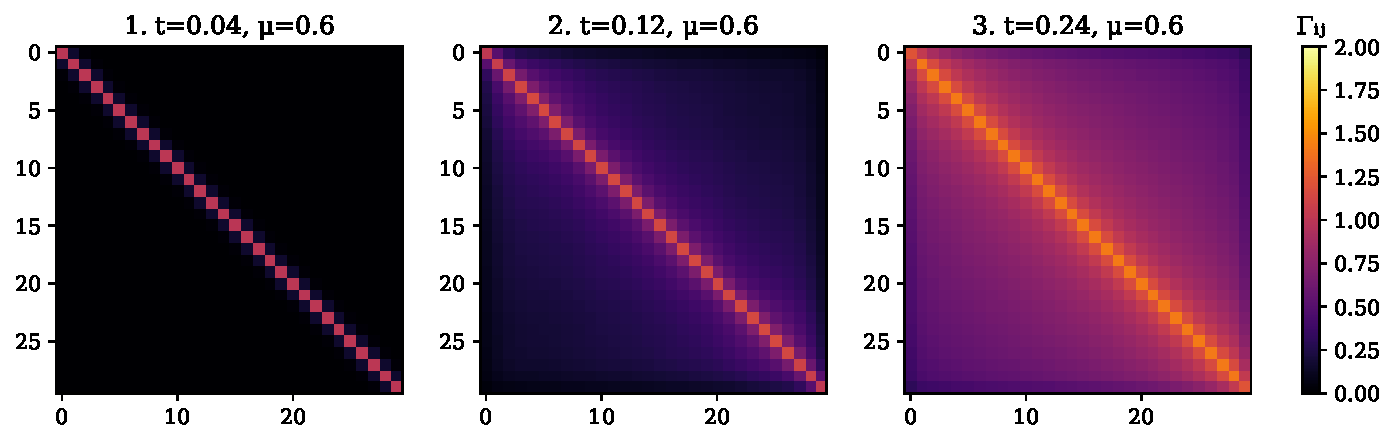
\includegraphics[width=\linewidth]{imgs/corrs.pdf}
\caption{The characteristic form of $\Gamma_{ij}$ at three points in the phase space: MI (1), critical point (2), and SF (3). The same points are used for illustration purposes throughout the text.}
\label{fig:corrmat}
\end{figure}

\section{Methodology}


In this article, we will focus on three key quantities to distinguish between these phases: the correlation length $\xi$, the average site occupancy $\langle n_j \rangle$, and the polynomial degree \( K \) with which \(\Gamma^2\) decays, following the approach in [1]. These properties provide valuable insights into the nature of the MI and SF phases. By examining these parameters, we aim to deepen our understanding of the phase transitions within the one-dimensional Bose-Hubbard model.




 \frametitle{Intro}}

\frame{




\begin{minipage}{0.55\textwidth}
	The graph is given via
    \begin{itemize}
        \iitem{target vertex $V_0$}
        \iitem{available moves $\{\sigma_j\}$}
    \end{itemize}
\end{minipage}
\hfill
\begin{minipage}{0.37\textwidth}
    \begin{figure}[h]
	    \centering
	    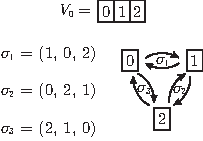
\includegraphics{imgs/pAsset 2.pdf}
	    %\caption{}
	    %\label{fig:}
	\end{figure}
\end{minipage}

\vfill

\begin{minipage}{0.6\textwidth}
	Graph structure:
    \begin{itemize}
    	\iitem{distance \\ $d(V)$ $\overset{\mathrm{def}}{=} \min\limits_{\text{path}} \text{len}\, \text{path}(V, V_0)$}
        \iitem{ring $d'$ $\overset{\mathrm{def}}{=} \{V \mid d(V) = d'\}$}
        \iitem{$V_0$ eccentricity $\overset{\mathrm{def}}{=} \max\limits_V d(V)$ \\ (may be the same as diameter $D$)} 
    \end{itemize}
\end{minipage}
\hfill
\begin{minipage}{0.37\textwidth}
    \begin{figure}[h]
	    \centering
	    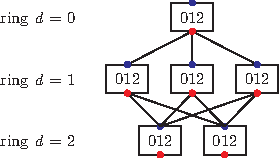
\includegraphics{imgs/pAsset 3.pdf}
	    %\caption{}
	    %\label{fig:}
	\end{figure}
\end{minipage}


 \frametitle{Problem statement}}

\frame{

\begin{itemize}
    \iitem{state as vector of numbers $(0, 0, 0, 0, 1, 1, 1, 1, \ldots)$}
    \iitem{permutations behave as}
    \begin{equation*}
        f_0 = \begin{pmatrix}
            0 & 1 & 2 & 3 & \ldots\\
            0 & 1 & 19 & 17 & \ldots\\
        \end{pmatrix}
    \end{equation*}
\end{itemize}

\begin{figure}[h]
    \centering
    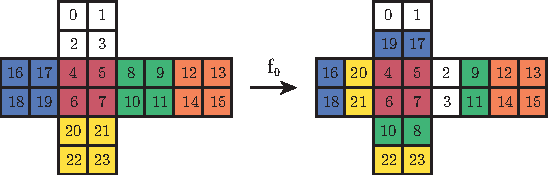
\includegraphics{imgs/pAsset 1.pdf} \vspace{5mm}
    \caption{Example of permutation, code \href{https://www.kaggle.com/code/marksix/visualize-allowed-moves}{here}}
    %\label{fig:}
\end{figure}
 \frametitle{Example: Rubik's Cube}}

\frame{
\begin{itemize}
	\iitem{for Cayley graphs the vertex degree is $n = \card\{\sigma_j\}$}
	\iitem{as a consequence exponential growth $\card \text{ring}\, d' \propto n^{d'}$
	}
\end{itemize}


\begin{table}[h!]
    \centering
    \begin{tabular}{ccccc}
        \toprule
        & 2x2 & 3x3 & 4x4 & 5x5 \\
		\midrule
        Rubik's Cube & $3.7 \times 10^{6}$ & $4.3 \times 10^{19}$ & $7.4 \times 10^{45}$ & $2.8 \times 10^{74}$ \\
        Sliding Puzzle & $1.2 \times 10^{1}$ & $1.8 \times 10^{5}$ & $1.0 \times 10^{13}$ & $7.8 \times 10^{24}$ \\
        \bottomrule
    \end{tabular}
    \caption{Graph sizes for different puzzles}
\end{table}



\begin{table}[h!]
\centering
\begin{tabular}{@{} lcccc @{}}
    \toprule
    & 2x2 & 3x3 & 4x4 & 5x5 \\
    \midrule
    Rubik's Cube & $14$ & $26$ & $\approx 48$ & $\approx 80$ \\
    Sliding Puzzle & $4$ & $31$ & $80$ & $\approx 150$ \\
    \bottomrule
\end{tabular}
\caption{Graph diameters for different puzzles}
\end{table} \frametitle{Scale of the disaster}}

\frame{
\only<1,2,3>{
\begin{tikzpicture}[remember picture,overlay]
    \node[anchor=north west, rotate=0, gray, font=\small] at (-1,-7.2) {
    [1] S. McAleer et al., Solving the rubik’s cube with approximate policy iteration
    };
\end{tikzpicture}
}


\begin{minipage}{0.62\textwidth}
\only<1>{
	Data annotation by  Bellman Equation:
	\begin{enumerate}
		\item $d(V_2) = d(V_0) + 1 = 1$
		\item $d(V_4) = d(V_2) + 1 = 2$
		\item $d(V_5) = d(V_4) + 1 = 3$
		\item $d(V_1) = d(V_5) + 1 = 4$ \\ $d(V_6) = d(V_5) + 1 = 4$
	\end{enumerate}
}
\only<2, 3>{
	Model $J(V)$ is trained to predict $d$. \vspace{5mm}

	Until convergence repeat:
    \begin{itemize}
        \iitem{for $V \in \text{dataset}$ calculate $J'(V)$}
        \iitem{train model to predict $J'(V)$}
    \end{itemize}
    \vspace{5mm}
    
    \only<3>{
	Important details:
    \begin{itemize}
        \iitem{dataset generation}
        \iitem{model architecture}
        \iitem{vertex representation}
        \iitem{model-based pathfinding}
    \end{itemize}
    }


}
\end{minipage}
\hfill
\begin{minipage}{0.36\textwidth}
Bellman equation: \vspace{-2mm}
\begin{equation*}
	\phantom{42} \hfill \boxed{J'(V) = 1 + \min_\sigma J(\sigma V)}
\end{equation*}
\vspace{-10mm}

\begin{figure}[h]
    \centering
    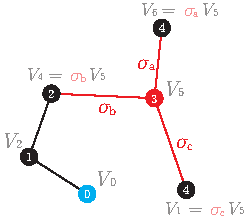
\includegraphics{imgs/pAsset 4.pdf}
    %\caption{}
    %\label{fig:}
\end{figure}


\end{minipage}

\only<2>{
\vfill 
Instead of storing a dictionary with all the vertices, we train the model to <<remember>>/<<understand>> the values found according to Bellman.
} \frametitle{Deep Approximate Value Iteration (DAVI)}}

\frame{
% {{0, 1, 1},
% {1, 18, 18},
% {2, 243, 243},
% {3, 3240, 3240},
% {4, 43254, 43239},
% {5, 577368, 574908},
% {6, 7706988, 7618438},
% {7, 102876480, 100803036},
% {8, 1373243544, 1332343288},
% {9, 18330699168, 17596479795},
% {10, 244686773808, 232248063316},
% {11, 3266193870720, 3063288809012},
% {12, 43598688377184, 40374425656248},
% {13, 581975750199168, 531653418284628},
% {14, 7768485393179328, 6989320578825358},
% {15, 103697388221736960, 91365146187124313},
% {16, 1384201395738071424, 1100000000000000000},
% {17, 18476969736848122368, 12000000000000000000},
% {18, 246639261965462754048, 29000000000000000000},
% {19, 3292256598848819251200, 1500000000000000000},
% {20, 43946585901564160587264, 300000000}}

% квинтиллионом


For balanced dataset, we do $K \in [1, \sub{D}{est}]$ random steps from $V_0$.
\vfill

\begin{minipage}{0.55\textwidth}
It is important to carefully choose $\sub{K}{max} \sim \sub{D}{est}$.
    \begin{figure}[h]
        \centering
        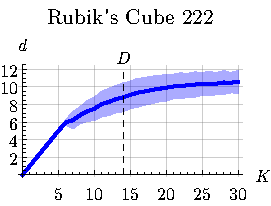
\includegraphics{imgs/dK_dist.pdf}
        %\caption{}
        %\label{fig:}
    \end{figure}
    
\end{minipage}
\hfill
\begin{minipage}{0.4\textwidth}
	\begin{figure}[h]
	    \centering
	    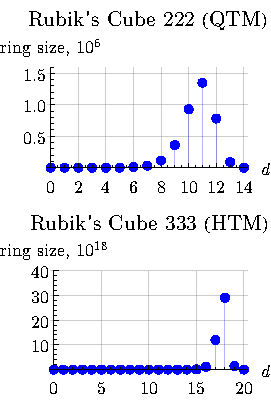
\includegraphics{imgs/d_dist.pdf}
	    %\caption{}
	    %\label{fig:}
	\end{figure}
\end{minipage}


 \frametitle{Dataset generation}}

% \frame{ %2Do
% \input{slides/models.tex} \frametitle{Model architecture: NN \& Boosting}}

% \frame{ %2Do
% % \begin{itemize}
% 	\iitem{one-hot encoding}
% 	\iitem{...}
% \end{itemize} \frametitle{Vertex representation}}

\frame{ %2Do
The cost of each node $V$ in the search tree:
\begin{equation*}
	f(V) = 
	\only<7>{\textcolor{blue}{\lambda}} 
	g(v) + h(V), 
	\hspace{5 mm} 
	\text{with }
	\left[\begin{aligned}
	    &g(v) &\text{ path cost} \\
	    &h(v) &\text{ heuristic function} \\
	\end{aligned}\right.
\end{equation*}

\begin{minipage}{0.55\textwidth}

\begin{beamerboxesrounded}[upper=block title, lower=block body,shadow=true]{\underline{A* algorithm}}
while $\sub{V}{n} \neq V_0$:
\begin{enumerate}
	\item $\sub{V}{n} = \argmin\limits_{V \in \text{queue}} f(V)$
	\item for $\sigma \in \{\sigma_j\}$: \\
	\hspace{5mm} if $g(V_n)+1 < g(\sigma V_n)$: \\
	\hspace{10mm} extend queue with $\sigma \sub{V}{n}$ \\
	\hspace{10mm} upd $g(\sigma \sub{V}{n}) = g(\sub{V}{n}) + 1$
\end{enumerate}
\end{beamerboxesrounded}

\end{minipage}
\hfill
\begin{minipage}{0.37\textwidth}
    \begin{figure}[h]
	    \centering
	    \only<1>{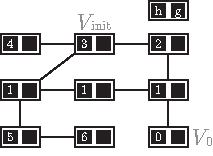
\includegraphics{imgs/pAsset 11.pdf}}
	    \only<2>{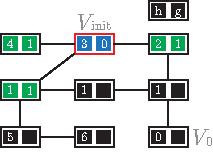
\includegraphics{imgs/pAsset 12.pdf}}
	    \only<3>{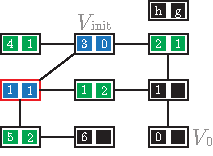
\includegraphics{imgs/pAsset 13.pdf}}
	    \only<4>{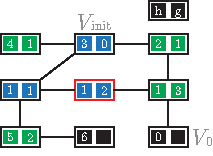
\includegraphics{imgs/pAsset 14.pdf}}
	    \only<5>{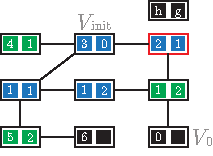
\includegraphics{imgs/pAsset 15.pdf}}
	    \only<6>{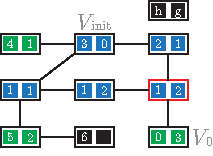
\includegraphics{imgs/pAsset 16.pdf}}
	    \only<7>{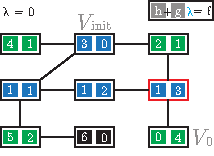
\includegraphics{imgs/pAsset 19.pdf}}
	    %\caption{}
	    %\label{fig:}
	\end{figure}
\end{minipage}

\phantom{42}

The path is guaranteed to be the shortest if $h(V) \leq d(V)$!

 \frametitle{Heuristic guided path search: A*}}

\frame{ %2Do
\begin{itemize}
	\iitem{Hamming distance (number of correct tiles)}
	\iitem{Manhattan distance\only<1, 2>{. For Sliding Puzzle 3х3 (180k states)}
	\only<1>{
		\begin{figure}[h]
		    \centering
		    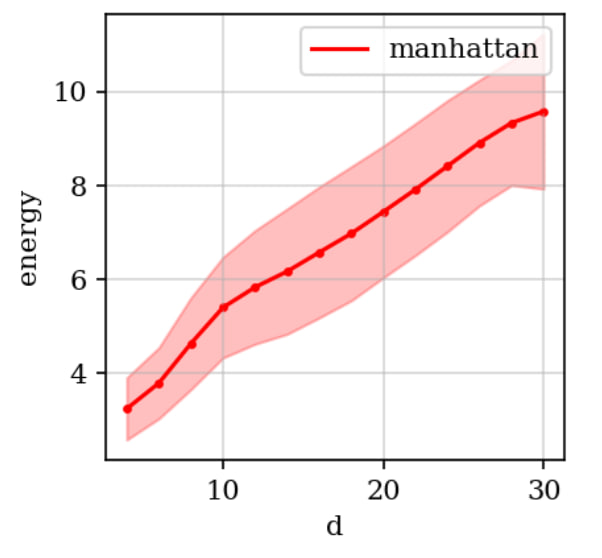
\includegraphics[width=0.35\textwidth]{imgs/manh.png}
		    %\caption{}
		    %\label{fig:}
		\end{figure}
		}
	\only<2>{
		\begin{figure}[h]
		    \centering
		    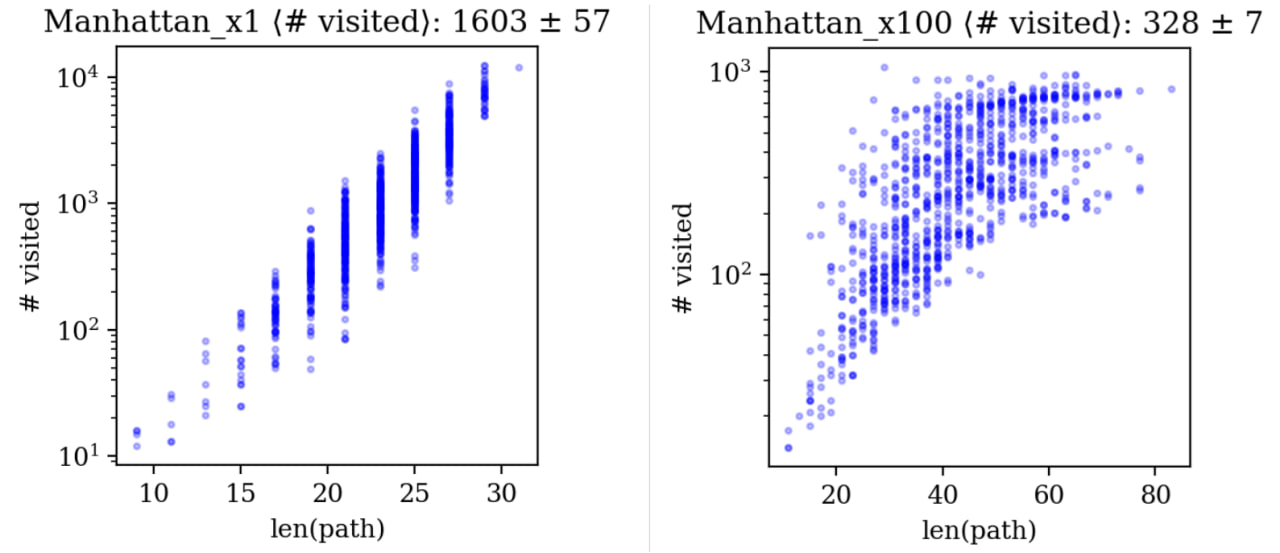
\includegraphics[width=0.75\textwidth]{imgs/15_1.png}
		    %\caption{}
		    %\label{fig:}
		\end{figure}
		}
	}
	\iitem{K-prediction
	\only<3>{
		\begin{figure}[h]
		    \centering
		    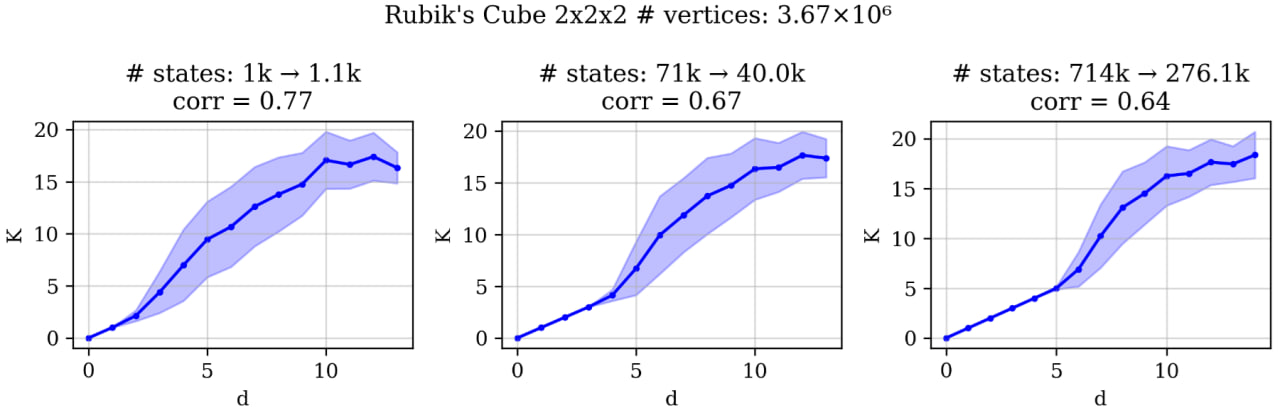
\includegraphics[width=0.99\textwidth]{imgs/222.png}
		    %\caption{}
		    %\label{fig:}
		\end{figure}
}
	}
	\iitem{KL-div*}
\end{itemize} \frametitle{Heuristics}}

\frame{ %2Do
\begin{tikzpicture}[remember picture,overlay]
    \node[anchor=north west, rotate=0, gray, font=\small] at (-0.75,-7.2) {
    [3] K. Takano, Self-Supervision is All You Need for Solving Rubik’s Cube, 2023
    };
\end{tikzpicture}

\vspace{-5mm}
\begin{itemize}
	\iitem model is trained to predict probability distribution of the source vertex
	\iitem the shorter a path, the more likely it is to occur randomly
	\iitem the cumulative probability $p_1 p_2 \ldots$ of a random training scramble increases as the number of moves decreases.
	\iitem beam search (greedy algorithm) based on cumulative $p$
\end{itemize}
% \vspace{-3mm}

% Fundamental property of combinatorial search: 

\begin{figure}[h]
    \centering
    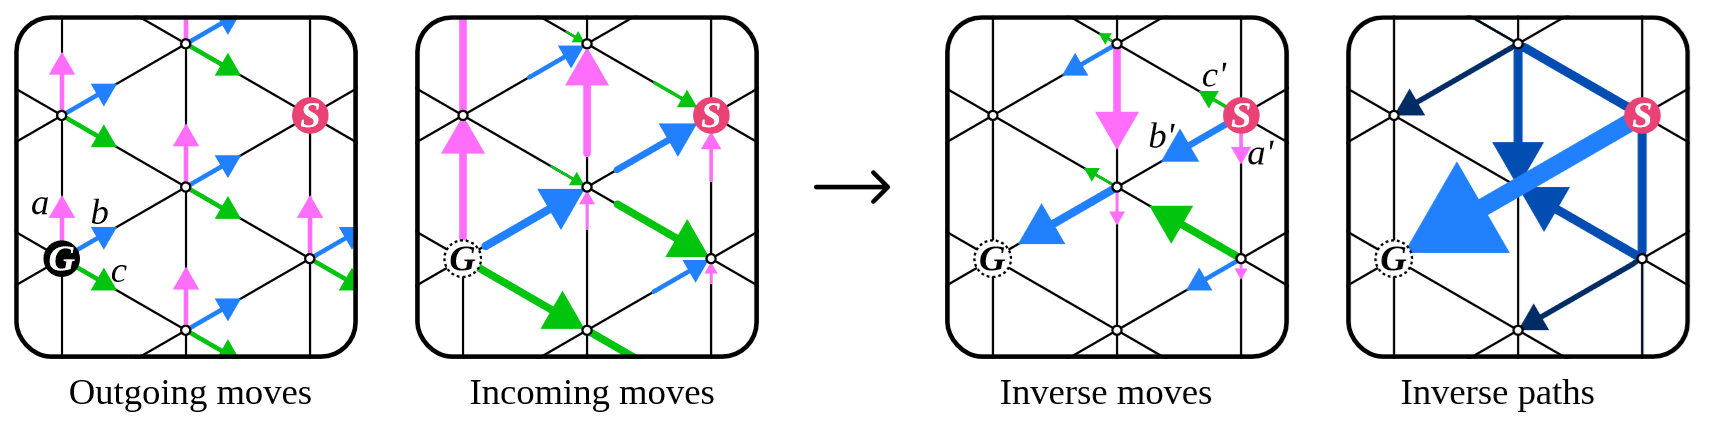
\includegraphics[width=1.0\textwidth]{imgs/unscrambling.png}
    \caption{A miniature instance of combinatorial search with a predefined goal from [3].}
    %\label{fig:}
\end{figure}


 \frametitle{Unscrambling}}

\frame{ %2Do
Movement on a graph with heuristics $h$ as a process of searching for a state with the lowest energy $E(V) = h(V)$.

% \phantom{42}


\begin{minipage}{0.53\textwidth}
\only<1,2>{
\begin{beamerboxesrounded}[upper=block title, lower=block body,shadow=true]{\underline{Metropolis-Hastings algorithm}}
init $V = V_0$ \\
while $V \neq V_0$:
\begin{enumerate}
	\item Choose a random $\sigma \in {\sigma_j}$
	\item if $E(\sigma V)$ < $E(V)$: \\ \hspace{5 mm} $V= \sigma V$
	\item else with $p = e^{- \beta(E(\sigma V) - E(V))}$ \\ \hspace{5 mm} $V= \sigma V$
\end{enumerate}
\end{beamerboxesrounded}
}
\only<3>{
	\begin{figure}[h]
	    \centering
	    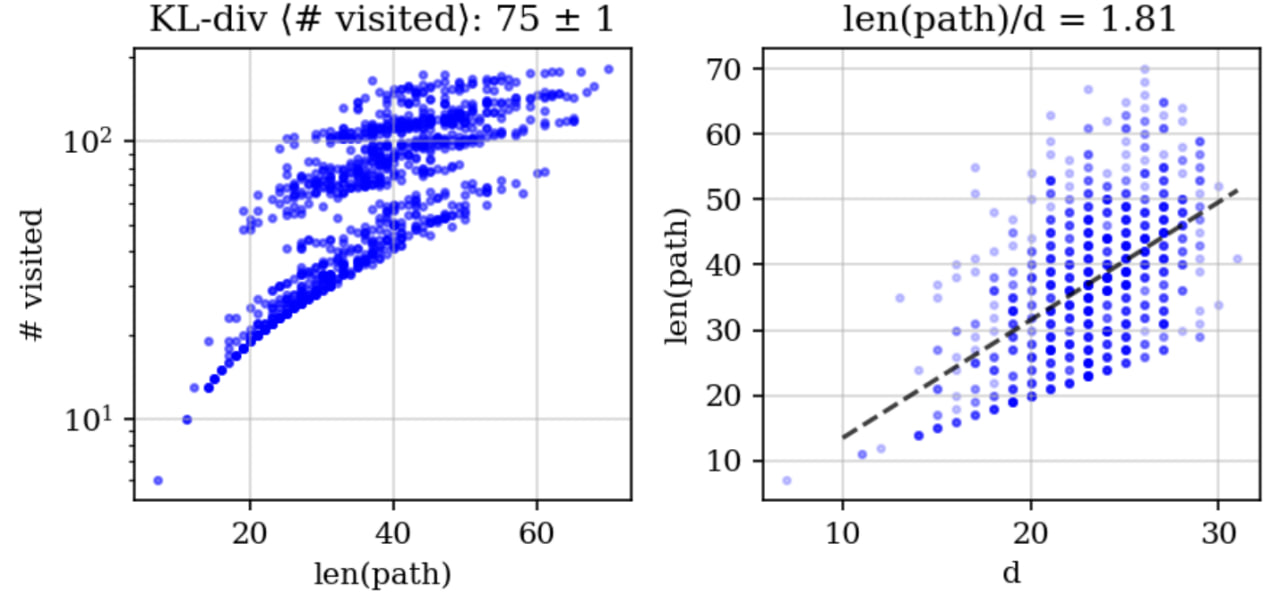
\includegraphics[width=1\textwidth]{imgs/t3.png}
	    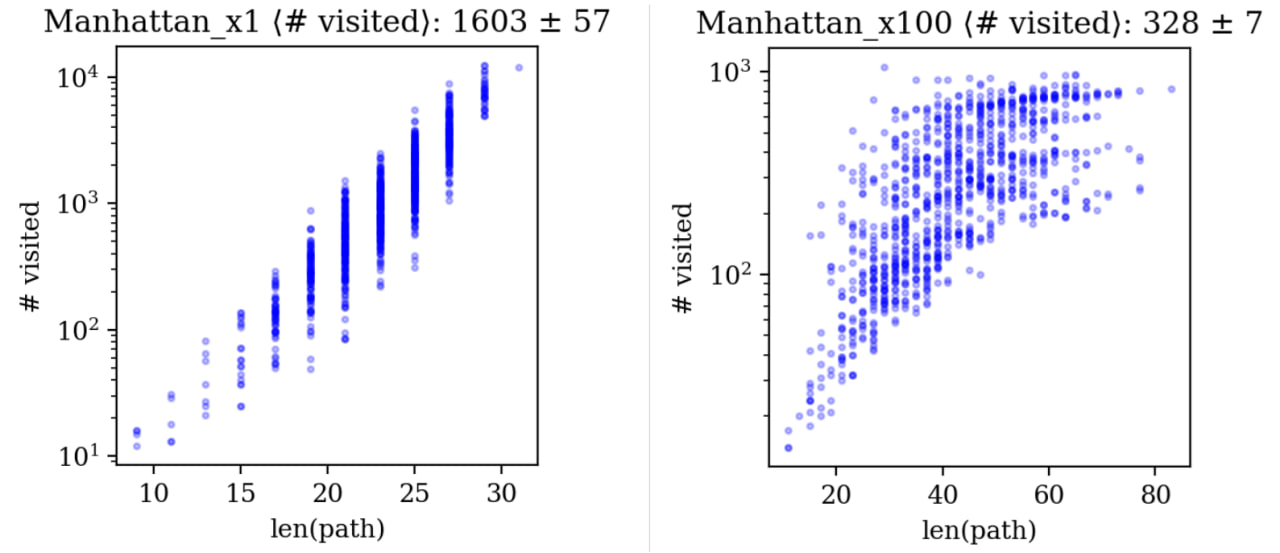
\includegraphics[width=1\textwidth]{imgs/15_1.png}
	    %\caption{}
	    %\label{fig:}
	\end{figure}
}
\end{minipage}
\hfill
\begin{minipage}{0.43\textwidth}
\onslide<2,3>{
    \begin{figure}[h]
	    \centering
	    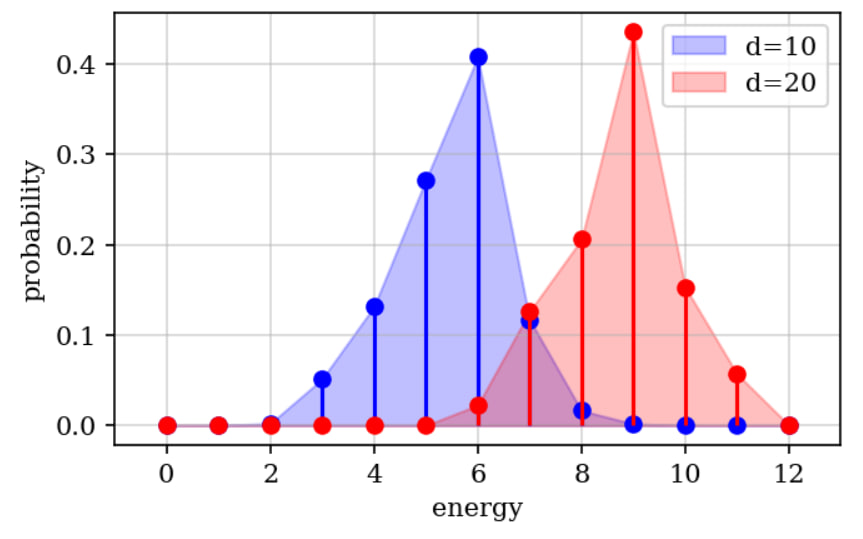
\includegraphics[width=1\textwidth]{imgs/t1.png}
	    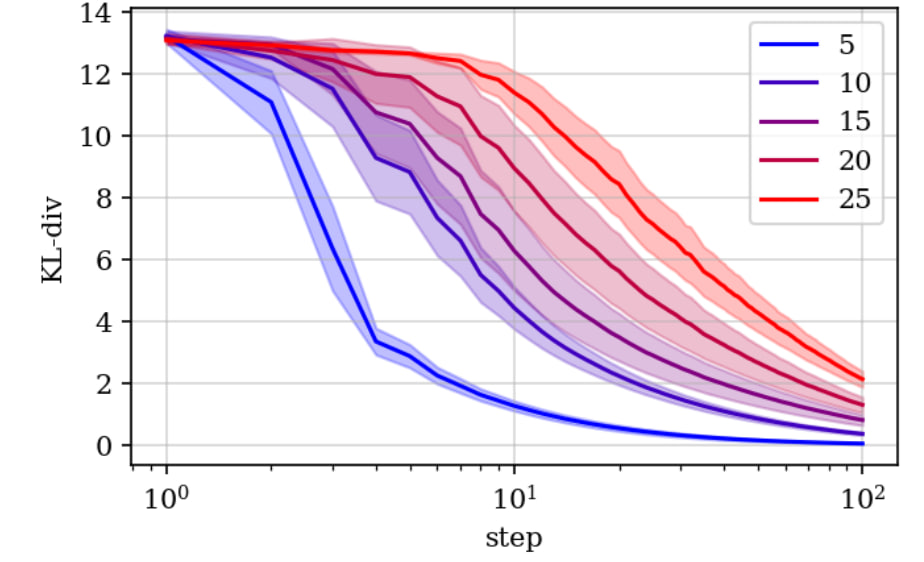
\includegraphics[width=1\textwidth]{imgs/t2.png}
	    %\caption{}
	    %\label{fig:}
	\end{figure}
}
\end{minipage}

% \phantom{42}

The behavior is highly dependent on the inverse temperature $\beta$. 

 \frametitle{Metropolis-Hastings algorithm}}

% \frame{ %2Do
% \begin{figure}[h]
    \centering
    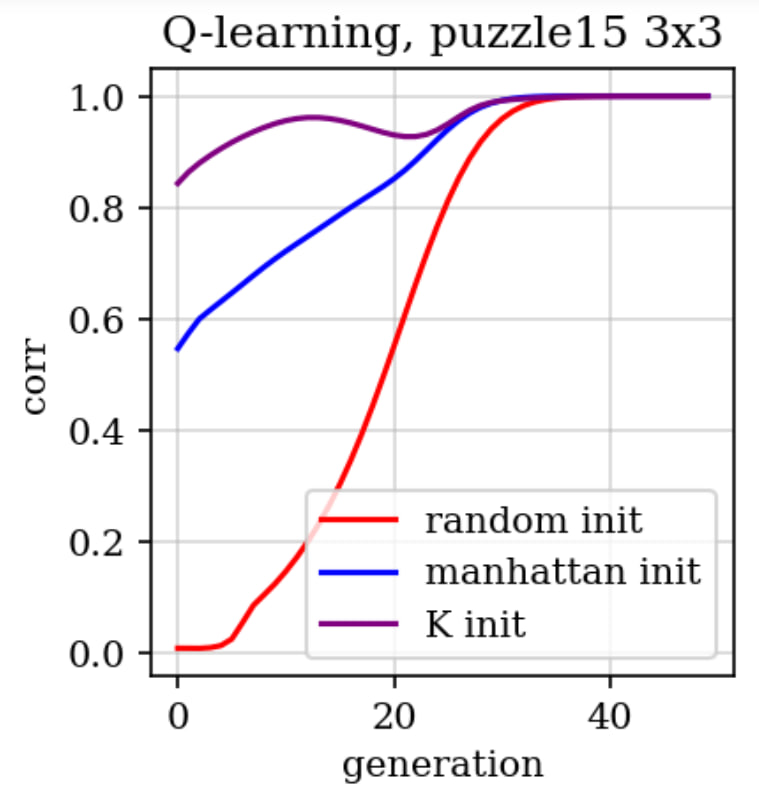
\includegraphics[width=0.5\textwidth]{imgs/t5.png}
    %\caption{}
    %\label{fig:}
\end{figure}
 \frametitle{Bellman update}}

% \frame{
%  \begin{tikzpicture}[overlay, remember picture]
        \node[circle, fill=black, inner sep=2pt, label=above:$A$] at (current page.north east) [xshift=-2cm, yshift=-2cm] (A) {};
        \node[circle, fill=black, inner sep=2pt, label=above:$B$] at (current page.north east) [xshift=-1cm, yshift=-2cm] (B) {};
        \draw (A) -- (B);
\end{tikzpicture}



\begin{itemize}
    \iitem  Pure states $\ket{\psi_{AB}}$: 
        \begin{itemize}
            \iitem{\textit{Product state} if $\ket{\psi_{AB}} = \ket{\psi_A} \otimes \ket{\psi_B}$}
            \iitem{$A$ is entangled with $B$ otherwise}
        \end{itemize}
    \vspace{3mm}
    \iitem Mixed states $\hat{\rho}_{AB}$
    \begin{itemize}
        \iitem{\textit{Separable state} if $\hat{\rho}_{AB} = \sum_k p_k \hat{\rho}_A^k \otimes \hat{\rho}_B^k$}
        \iitem{$A$ is entangled with $B$ otherwise}
    \end{itemize}
\end{itemize}

\vfill

\begin{figure}[h]
    \centering
    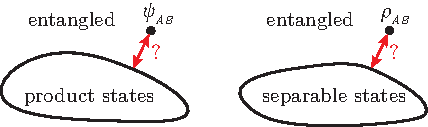
\includegraphics{imgs/Asset 2.pdf}
    %\caption{}
    %\label{fig:}
\end{figure}


% \begin{minipage}{0.45\textwidth}
%     \begin{block}{Entangled}
        
%     \end{block}
% \end{minipage}
% \hfill
% \begin{minipage}{0.45\textwidth}
%     \begin{block}{Non-entangled states}
%         For pure states: 
%     \end{block}
% \end{minipage}
%      \frametitle{States}}


% \frame{
%  \begin{tikzpicture}[overlay, remember picture]
        \node[circle, fill=black, inner sep=2pt, label=above:$A$] at (current page.north east) [xshift=-2cm, yshift=-2cm] (A) {};
        \node[circle, fill=black, inner sep=2pt, label=above:$B$] at (current page.north east) [xshift=-1cm, yshift=-2cm] (B) {};
        \draw (A) -- (B);
\end{tikzpicture}


\only<1,2>{
    \onslide<1,2>{
        Is this state entangled?
        \begin{equation*}
            \ket{\psi_{AB}} = \tfrac{1}{\sqrt{2}}\left(\ket{00} + \ket{01}\right)
        \end{equation*}
    }
    \onslide<2>{
    Of course not:
    \begin{equation*}
        \ket{\psi_{AB}} = \ket{0} \otimes \frac{1}{\sqrt{2}} \left(\ket{0}+ \ket{1}\right)
    \end{equation*}
    }
}
\only<3,4,5,6>{
    \onslide<3,4,5,6>{
    What about this?
    \begin{equation*}
        \ket{\psi_{AB}} = \tfrac{1}{2}\left(\ket{00} + \ket{10} - \ket{01} - \ket{11}\right)
    \end{equation*}
    }
    \onslide<4,5,6>{
    After some SVD (or \textbf{Schmidt decomposition}):
    \begin{equation*}
        \ket{\psi_{AB}} = \sum_{a \in A} \sum_{b \in B} \psi_{ab} \ket{a} \otimes \ket{b} = \sum_a \sum_b \frac{1}{2}\begin{pmatrix}
        1 & -1 \\
        1 & -1 \\
    \end{pmatrix}_{ab}
     \ket{ab}
    \end{equation*}
    }
    \only<5>{
        \begin{equation*}
        U \begin{pmatrix}
            \sqrt{\lambda_1} & 0 \\
            0 & \sqrt{\lambda_2} \\
        \end{pmatrix} V = 
        \frac{1}{\sqrt{2}}\begin{pmatrix}
        1 & . \\
        1 & . \\
        \end{pmatrix}
        \begin{pmatrix}
        1 & 0 \\
        0 & 0 \\
        \end{pmatrix}
        \frac{1}{\sqrt{2}}
        \begin{pmatrix}
        1 & . \\
        -1 & . \\
        \end{pmatrix}
        =
        \frac{1}{2}
        \begin{pmatrix}
        1 & -1 \\
        1 & -1 \\
        \end{pmatrix}       
        \end{equation*}
    }
    \only<6>{
        \begin{equation*}
            \ket{\psi_{AB}} = \tfrac{1}{\sqrt{2}} \left(\ket{0} + \ket{1}\right) \otimes \tfrac{1}{\sqrt{2}} \left(\ket{0} - \ket{1}\right)
        \end{equation*}
        We can see, that it is separable.
    }
}
\only<7>{
    Schmidt decomposition
    \begin{equation*}
        \ket{\psi_{AB}} = \sum_{a \in A} \sum_{b \in B} \psi_{ab} \ket{a} \otimes \ket{b} = \sum_j \sqrt{\lambda_j} \ket{\psi_{A,j}} \ket{\psi_{B,j}}
    \end{equation*}
    feeply connected with the reduced density matrix $\rho_{A,B}$
    \begin{equation*}
        \rho_{B, A} = \tr_{A,B} \left(\ket{\psi_{AB}}\right) = \sum_{i} \lambda_i \kb{\psi_{B,A}}{\psi_{B,A}}.
    \end{equation*}

    If there is no entanglement, than 
    \begin{equation*}
        \rho_{A,B} = \kb{\psi_{A,B}}{\psi_{A,B}} 
    \end{equation*}
} \frametitle{Bipartite entanglement in pure states: SVD}}


% \frame{
%  \begin{tikzpicture}[overlay, remember picture]
        \node[circle, fill=black, inner sep=2pt, label=above:$A$] at (current page.north east) [xshift=-2cm, yshift=-1.5cm] (A) {};
        \node[circle, fill=black, inner sep=2pt, label=above:$B$] at (current page.north east) [xshift=-1cm, yshift=-1.5cm] (B) {};
        \draw (A) -- (B);
\end{tikzpicture}

The Entanglement of Formation  defined throught \textit{convex roof}:
\begin{equation*}
	E_F(\rho_{AB}) \overset{\mathrm{def}}{=} \min_{\{p_j, \psi_j\}} \sum_j p_j S(\rho_{A,j}), 
\end{equation*}
with $\rho_{AB} = \sum_j p_j \kb{\psi_j}{\psi_j}$ and $\rho_{A,j} = \tr_B \kb{\psi_j}{\psi_j}$.


\onslide<2>{
	\phantom{42}

	For two qubits:
	\begin{equation*}
		E_F(\rho) = - \sum_{\sigma = \pm} \tfrac{1}{2}\sqrt{1+\sigma C^2(\rho)} \ln \tfrac{1}{2}\sqrt{1 + \sigma C^2(\rho)},
	\end{equation*}
	$C(\rho) \in [0, 1]$ -- \textit{concurrence}, that can be calculated from $R = \sqrt{\rho} \tilde{\rho} \sqrt{\rho} = \sqrt{\rho} (\sigma_y \otimes \sigma_y) \rho^* (\sigma_y \otimes \sigma_y)$ with $\lambda_1^2 \geq \ldots \geq \lambda_4^2$
	\begin{equation*}
		C = \max(\lambda_1 - \lambda_2 - \lambda_3 - \lambda_4, 0).
	\end{equation*}
} \frametitle{Entanglement in mixed states: EoF}}


% Concurrence, tau 1, tau 2     <=>    EXP I 
% 

% https://www.kaggle.com/code/marksix/visualize-allowed-moves
% \begin{thebibliography}{9}
% \bibitem{rokicki2014} T. Rokicki et al.,  The diameter of the Rubik's cube group is twenty, 2014.
% \bibitem{chris} Chris Hardwick, The Diameter of the 4x4x4 and 5x5x5 Cube, 2008.
% \bibitem{puzzle2x2} Wikipedia, \textit{15 puzzle}, \url{https://en.wikipedia.org/wiki/15_puzzle}, accessed 2024.
% \bibitem{puzzle3x3} Erik D. Demaine, 8 puzzle and 15 puzzle, accessed 2024.
% \bibitem{puzzle4x4} G. Wilson, \textit{Graph Diameters for Sliding Puzzle}, \url{http://www.mathematische-basteleien.de/slidingpuzzle.htm}, accessed 2024.
% \bibitem{puzzle5x5} J. Tromp and G. Farnebäck, \textit{Combinatorial and computational aspects of the 24 puzzle}, \url{https://tromp.github.io/puzzle24/puzzle24.html}, 2006.
% \end{thebibliography}

\end{document}

